\documentclass[10pt]{beamer}
\usepackage{tikz}
\usetikzlibrary{shapes.geometric, arrows.meta, positioning}
\usepackage{amsmath}

\title{NLP Patient Description to Acuity}
\subtitle{Deep Learning and Mathematical Triage}
\author{Hospital Triage AI Project}
\date{\today}

\begin{document}
	
	\begin{frame}
		\titlepage
	\end{frame}
	
	% --- SLIDE 1 ---
	\begin{frame}{The Clinical Scenario}
		\begin{center}
			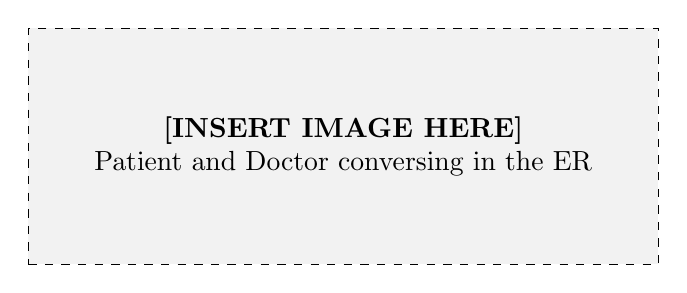
\begin{tikzpicture}
				\node[draw, dashed, fill=gray!10, minimum width=8cm, minimum height=3cm, align=center] (img1) {
					\textbf{[INSERT IMAGE HERE]}\\
					Patient and Doctor conversing in the ER
				};
			\end{tikzpicture}
		\end{center}
		
		\vspace{0.5cm}
		\textbf{The Chief Complaint (Our Running Example):}\\
		\textit{"My chest feels like an elephant is sitting on it, and I can't catch my breath. The pain is crushing."} [cite: 2104]
		
		\vspace{0.2cm}
		How does a computer mathematically interpret this raw, unstructured human panic and convert it into a life-saving triage color?
	\end{frame}
	
	% --- SLIDE 2 ---
	\begin{frame}{The Dual Pathway: TEWS vs. NLP Chatbot}
		\begin{center}
			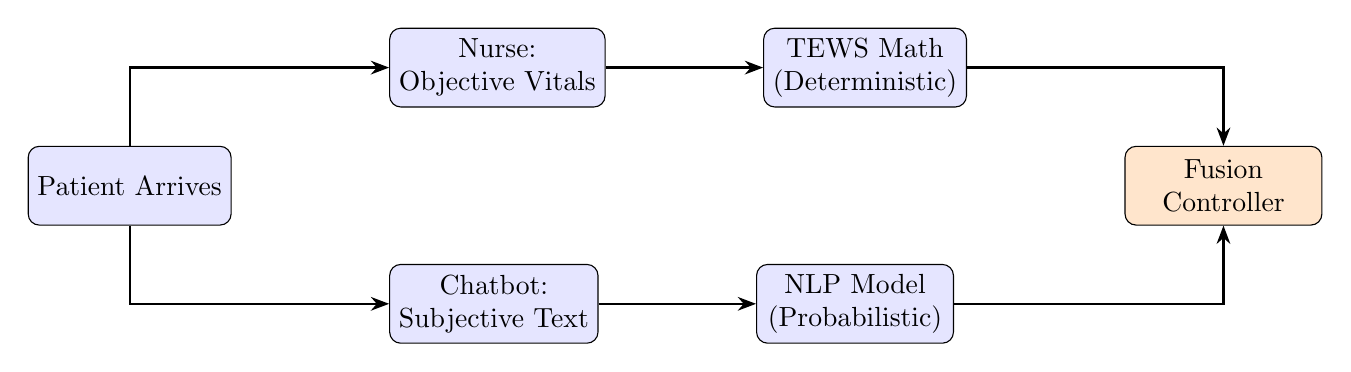
\begin{tikzpicture}[node distance=1.5cm and 2cm, auto,
				box/.style={draw, rounded corners, minimum width=2.5cm, minimum height=1cm, align=center, fill=blue!10},
				arrow/.style={-{Stealth}, thick}]
				
				\node[box] (start) {Patient Arrives};
				
				\node[box, right=of start, yshift=1.5cm] (nurse) {Nurse:\\Objective Vitals};
				\node[box, right=of nurse] (tews) {TEWS Math\\(Deterministic)};
				
				\node[box, right=of start, yshift=-1.5cm] (bot) {Chatbot:\\Subjective Text};
				\node[box, right=of bot] (nlp) {NLP Model\\(Probabilistic)};
				
				\node[box, right=of tews, yshift=-1.5cm, fill=orange!20] (fusion) {Fusion\\Controller};
				
				\draw[arrow] (start) |- (nurse);
				\draw[arrow] (nurse) -- (tews);
				\draw[arrow] (tews) -| (fusion);
				
				\draw[arrow] (start) |- (bot);
				\draw[arrow] (bot) -- (nlp);
				\draw[arrow] (nlp) -| (fusion);
			\end{tikzpicture}
		\end{center}
		
		\vspace{0.2cm}
		\begin{itemize}
			\item \textbf{Manual TEWS:} Objective mathematical baseline using vital signs[cite: 2190].
			\item \textbf{NLP Chatbot:} Processes subjective human text to catch critical red flags[cite: 2201].
		\end{itemize}
	\end{frame}
	
	% --- SLIDE 3 ---
	\begin{frame}{NLP Analysis: Supervised Deep Learning}
		\begin{center}
			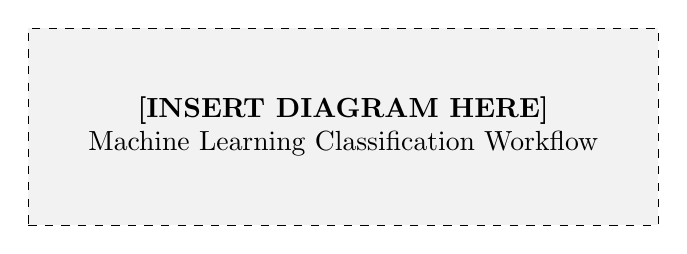
\begin{tikzpicture}
				\node[draw, dashed, fill=gray!10, minimum width=8cm, minimum height=2.5cm, align=center] (img2) {
					\textbf{[INSERT DIAGRAM HERE]}\\
					Machine Learning Classification Workflow
				};
			\end{tikzpicture}
		\end{center}
		
		\begin{itemize}
			\item \textbf{The Core Model:} We are using Supervised Learning to perform Text Classification[cite: 1949, 2101].
			\item \textbf{How it Helps:} The AI acts as the "supervisor," learning from historical patient records[cite: 1946]. It evaluates messy text and outputs strict probabilities for the 5 SATS categories (Red, Orange, Yellow, Green, Blue)[cite: 1949].
		\end{itemize}
	\end{frame}
	
	% --- SLIDE 4 ---
	\begin{frame}{Phase 1: Tokenization (Breaking it Down)}
		\begin{itemize}
			\item Computers cannot read English; they only understand numbers[cite: 1574].
			\item \textbf{Tokenization:} The model breaks the raw sentence down into smaller sub-word units called tokens[cite: 1576].
			\item \textbf{The Math:} It assigns a simple integer ID to each token based on a pre-existing dictionary[cite: 1603].
		\end{itemize}
		
		\vspace{0.3cm}
		\textbf{Example Assignment:}
		\begin{table}[]
			\begin{tabular}{|l|l|}
				\hline
				\textbf{Raw Word} & \textbf{Token ID} \\ \hline
				crushing          & 14592             \\ \hline
				chest             & 345               \\ \hline
				pain              & 890               \\ \hline
			\end{tabular}
		\end{table}
	\end{frame}
	
	% --- SLIDE 5 ---
	\begin{frame}{Phase 1: Embedding (Words to Coordinates)}
		\begin{center}
			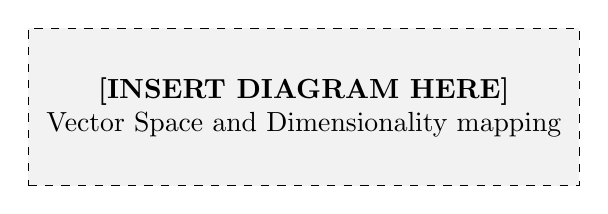
\begin{tikzpicture}
				\node[draw, dashed, fill=gray!10, minimum width=7cm, minimum height=2cm, align=center] (img3) {
					\textbf{[INSERT DIAGRAM HERE]}\\
					Vector Space and Dimensionality mapping
				};
			\end{tikzpicture}
		\end{center}
		
		\begin{itemize}
			\item A single ID number (like 345) does not tell the AI what "chest" actually means[cite: 1606].
			\item \textbf{The Conversion:} The model converts each discrete token into a dense, 768-dimensional mathematical vector[cite: 1578].
			\item \textbf{The Vector:} Think of a massive room with 768 axes. The word "chest" becomes a specific coordinate in that room: $[0.12, -0.45, 0.88, \dots, -0.01]$[cite: 1609, 1611].
		\end{itemize}
	\end{frame}
	
	% --- SLIDE 6 ---
	\begin{frame}{Contextual Mapping: Understanding Meaning}
		The model cannot assign random numbers; context dictates meaning[cite: 1612]. It calculates the exact vector using:
		
		$$E(t_{i}) = E_{word}(t_{i}) + E_{pos}(i) + E_{seg}(t_{i})$$ [cite: 1613]
		
		\begin{itemize}
			\item $E_{word}(t_{i})$: The base clinical concept of the word (e.g., "chest")[cite: 1613].
			\item $E_{pos}(i)$: The positional math. Because "chest pain" is fundamentally different from "pain in chest"[cite: 1614].
			\item $E_{seg}(t_{i})$: The segment embedding for multi-sentence logic[cite: 1615].
		\end{itemize}
	\end{frame}
	
	% --- SLIDE 7 ---
	\begin{frame}{The Matrix: What the Data Looks Like}
		The patient's entire sentence is stored as an $M \times D$ mathematical matrix[cite: 1616].
		\begin{itemize}
			\item \textbf{$M$ (Rows):} Sequence Length (number of tokens)[cite: 1642].
			\item \textbf{$D$ (Columns):} Embedding Dimension (768)[cite: 1644].
		\end{itemize}
		
		\vspace{0.2cm}
		\textbf{Example Matrix for "crushing chest pain" ($3 \times 768$):}
		\vspace{0.1cm}
		
		\begin{tabular}{|l|c|c|c|c|}
			\hline
			\textbf{Token} & $D_1$ & $D_2$ & $\dots$ & $D_{768}$ \\ \hline
			crushing & $0.94$ & $-0.11$ & $\dots$ & $0.05$ \\ \hline
			chest & $0.12$ & $-0.45$ & $\dots$ & $-0.01$ \\ \hline
			pain & $0.88$ & $0.33$ & $\dots$ & $0.62$ \\ \hline
		\end{tabular}
	\end{frame}
	
	% --- SLIDE 8 ---
	\begin{frame}{Phase 2: The 12 Transformer Layers}
		\begin{center}
			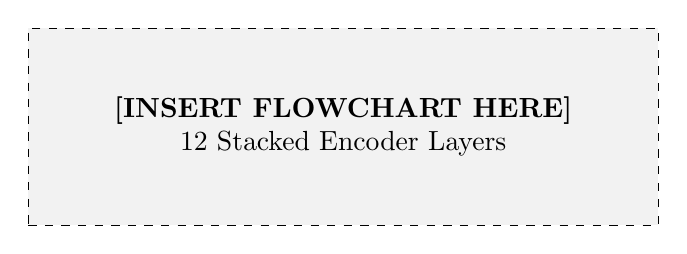
\begin{tikzpicture}
				\node[draw, dashed, fill=gray!10, minimum width=8cm, minimum height=2.5cm, align=center] (img4) {
					\textbf{[INSERT FLOWCHART HERE]}\\
					12 Stacked Encoder Layers
				};
			\end{tikzpicture}
		\end{center}
		
		\begin{itemize}
			\item \textbf{What is a Transformer?} A neural network architecture that abandoned left-to-right reading. It processes entire sentences in parallel[cite: 1988, 2072].
			\item \textbf{Deep Learning:} By stacking 12 encoder layers, the model moves from shallow word recognition to deep, abstract clinical understanding[cite: 1954].
		\end{itemize}
	\end{frame}
	
	% --- SLIDE 9 ---
	\begin{frame}{The Self-Attention Equation}
		From the paper "Attention Is All You Need"[cite: 1571]:
		
		$$Attention(Q,K,V) = \text{softmax}\left(\frac{QK^{\top}}{\sqrt{d_k}}\right)V$$ [cite: 1582]
		
		\textbf{The Parameters:}
		\begin{itemize}
			\item \textbf{$Q$ (Query):} The word currently being evaluated (e.g., "crushing")[cite: 1623].
			\item \textbf{$K$ (Key):} Every other word it compares against (e.g., "chest")[cite: 1624].
			\item \textbf{$V$ (Value):} The underlying meaning kept if deemed important[cite: 1625].
			\item \textbf{$QK^{\top}$ (Relevance):} The dot product calculating how strongly words align[cite: 1626].
			\item \textbf{$\sqrt{d_k}$ (Stabilizer):} Prevents the math from exploding and breaking the gradients[cite: 1628].
		\end{itemize}
	\end{frame}
	
	% --- SLIDE 10 ---
	\begin{frame}{The Probability Filter: Attention Weights}
		To figure out exactly how much mathematical weight to assign each word, the Softmax function is used[cite: 1583]:
		
		$$\alpha_{j}=\frac{\exp(e_{j})}{\sum_{k=1}^{m}\exp(e_{k})}$$ [cite: 1583]
		
		\begin{itemize}
			\item \textbf{$e_j, e_k$:} The raw, unconstrained mathematical scores[cite: 1632].
			\item \textbf{$\exp$:} Forces numbers to be positive and amplifies the differences between high and low scores[cite: 1633, 1634].
			\item \textbf{The Result ($\alpha_j$):} Suppresses filler words ("is", "my") and assigns massive percentage weight to clinical keywords ("crushing")[cite: 1584, 1636].
		\end{itemize}
	\end{frame}
	
	% --- SLIDE 11 ---
	\begin{frame}{How the AI Learns: Backpropagation}
		If the model guesses "Green" for a heart attack, how does it fix itself?
		
		\begin{itemize}
			\item \textbf{The Penalty (Loss):} The Cross-Entropy Loss formula calculates exactly how mathematically "wrong" the guess was compared to the true nurse label[cite: 2035].
			\item \textbf{The Investigation (Calculus):} Backpropagation uses calculus to travel backward through the 12 neural network layers[cite: 2038]. It computes derivatives to find exactly which random weights caused the error[cite: 2039].
			\item \textbf{The Correction (Optimization):} An optimizer calculates the gradient (slope of the error) and physically nudges the weights in the opposite direction[cite: 2041]. Next time, the guess is better[cite: 2042].
		\end{itemize}
	\end{frame}
	
\end{document}